\documentclass[%
 aip,
 jmp,%
 amsmath,amssymb,
%preprint,%
 reprint,%
%author-year,%
%author-numerical,%
]{revtex4-1}

\usepackage{longtable}     % helps with long table options
\usepackage{url}
\usepackage{graphicx}% Include figure files
\usepackage{dcolumn}% Align table columns on decimal point
\usepackage{bm}% bold math
\usepackage{geometry}[1in]
\usepackage{amsmath}
\usepackage{relsize}
\usepackage{lipsum}

\begin{document}
\author{K. Hoverson}
\author{M. Baker}
\author{N. Chrisman}
\author{T. Colburn}
\affiliation{
Arizona State University%\\This line break forced with \textbackslash\textbackslash
}%
\title[Linearity of ideal gas state variables]{Linearity of ideal gas state variables}
\date{\today}
\begin{abstract}
  Both the pressure of a fixed volume of gas and the volume of a gas at a fixed pressure were measured as a function of temperature. The relationship between these state variables was modeled using the ideal gas law. The data collected was used to approximate absolute zero Kelvin with respect to Celsius and confirm the linearity of the relationships between these state variables.
\end{abstract}
\keywords{Thermodynamics, ideal gas, constant pressure, constant temperature, gas thermometer}

\maketitle

\section{Introduction}

  The determination of absolute value by obtaining temperature readings of a volume of gas using two types of thermometers is the goal of this experiment.  By holding certain variables of the ideal gas law constant, the data was compared to the model to confirm the relationship of pressure, volume, and temperature.  The first thermometer holds atmospheric pressure constant and the change in volume will indicate the temperature. The second apparatus allows pressure to change while the volume is held at a constant. The measured temperature of the mass of air at a fixed volume should provide sufficient data for the linearity of the temperature as a function of pressure to be determined.

  The ideal gas law is:
  $$PV = nRT$$
  where $P$ is pressure, $V$ is volume, $n$ is the number of moles, $R$ is the universal gas constant, and $T$ is temperature. Should all these variables be measured with accuracy, the model is expected to provide enough data for a linear regression model to determine absolute zero temperature within a minimal margin of error.

\section{Procedure}
  \subsection{Experiment One}
  A constant pressure gas thermometer (similar FIG. 1) was used to test the linearity of the ideal gas law. This thermometer was composed of a long glass rod containing gas sealed at one end by a rubber stopper, and at the other end by a small quantity of mercury. Surrounding this inner chamber was a vestibule through which the authors were able to run water at various temperatures. During this process, the gas expanded or contracted, moving the mercury such that atmospheric pressure was maintained.

  The authors began by recording room temperature and the associated length of trapped gas in the thermometer. A steam generator was filled up halfway with water and heated by a hot plate to its boiling point. While the water was left to heat up, ice cold and warm water were independently run through the thermometer. A conventional metal thermometer was used to check the stability of the temperature of the fluid as it was passed through the device. Once it had sufficiently stabilized, the length of the trapped gas was recorded. This process was repeated during a third trial, wherein steam was passed through the vestibule.

  \begin{figure}[!h]
    \centering
    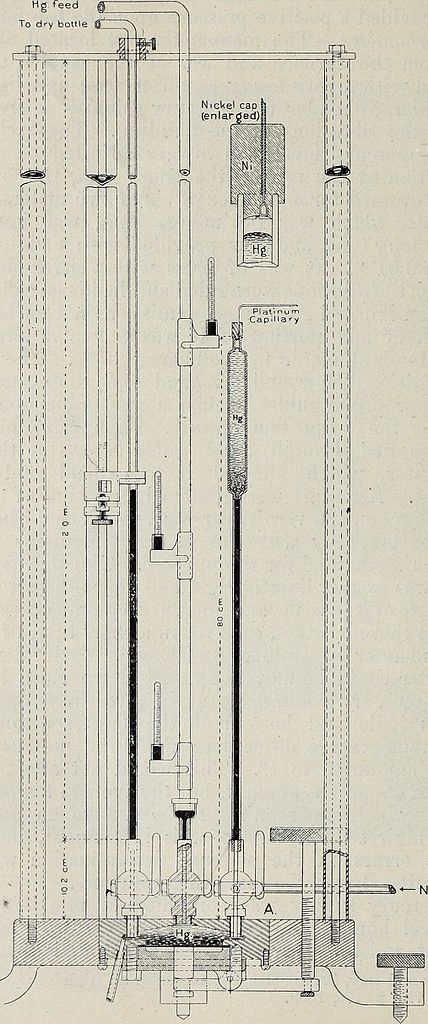
\includegraphics[scale=.3]{const_P_thermom.jpg}
    \caption{Constant pressure gas thermometer, similar to the apparatus used in experiment 1. A. L. Day and J. K. Clement, The American journal of science (1908).}
    \label{const_P}
  \end{figure}

  \subsection{Experiment Two}

  The linearity of the ideal gas law was tested once more, using a constant volume gas thermometer (FIG. 2). This apparatus was composed of a hollow, metal ball filled with gas, sealed by a valve and a pressure gauge measuring kiloPascals (kPa). A removable pressure release cap was fixed along the neck, such that the pressure of the gas inside was able to equilibrate to atmospheric conditions prior to experimentation.

  During each trial, the hollow metal ball was placed into either ice water, warm water, or boiling water, each contained by a steel beaker. Contact with the walls of the beaker was avoided. An electric thermometer was taped to the outside of the metal ball, and a glass thermometer was used to measure the temperature of the water during each trial. Once there was an observed stabilization of the ball temperature fluctuations around the water temperature, the pressure readings of the gauge were recorded.

  \begin{figure}[h]
    \centering
    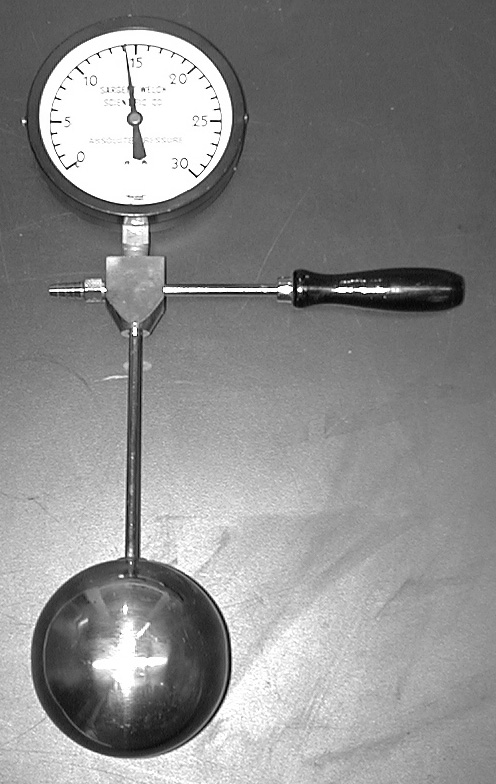
\includegraphics[scale=.95]{const_V_thermom.jpg}
    \caption{Constant Volume gas thermometer, similar to the apparatus used in experiment 2. D. Livelybrooks, University of Oregon.}
    \label{const_V}
  \end{figure}

  \section{Results}

  \subsection{Mercury Thermometer (constant pressure)}

  Four measurements were taken for water temperature and 1-dimensional volume (position of the mercury drop) for a total of 8 measurements. Pressure was held constant at 101.325 kPa as was the amount of gas, $n$.

  An initial volume of 61.5cm at a room temperature of 24$^{\circ}$C was recorded. The first container, filled with ice water, was poured in the funnel until the thermometer reached equilibrium. Volume of the mercury drop lowered to 57cm at a temperature of 7.5$^{\circ}$C. Warm water was poured into the funnel next, again giving the thermometer time to reach equilibrium. Once equilibrium was reached, the mercury drop had reached a volume of 66.1cm at a temperature of 45.5$^{\circ}$C. Following the hot water, steam was routed into the thermometer, giving a volume reading of 66.1cm and 98$^{\circ}$C. Figure 3 shows the plot of this data with a linear regression model.

  \begin{figure}[h]
    \centering
    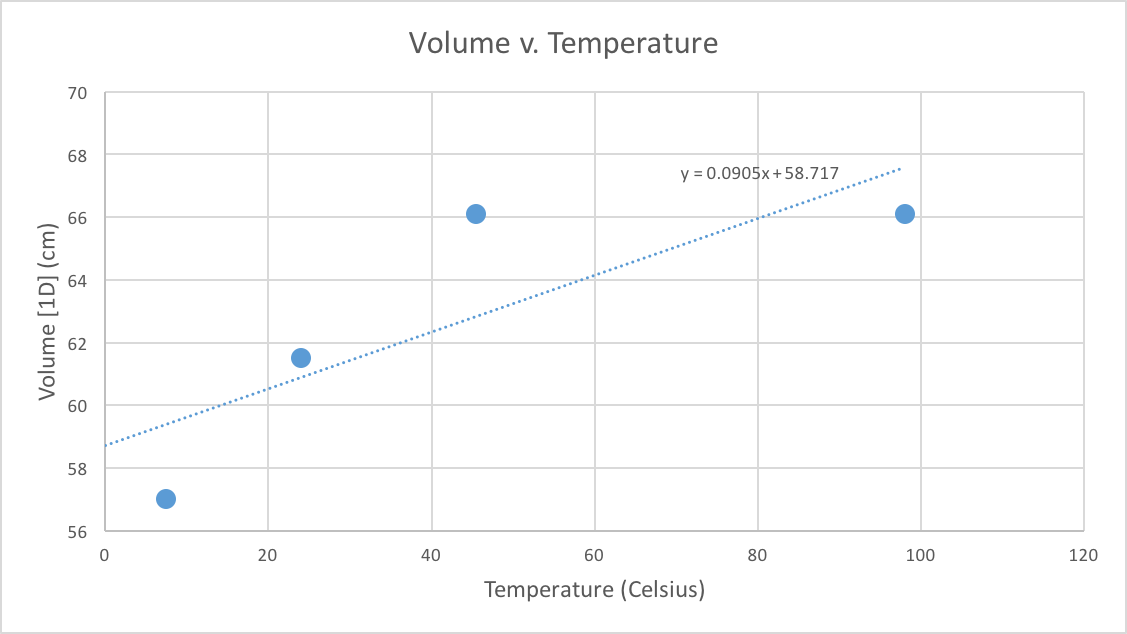
\includegraphics[scale=.4]{V_vs_T.png}
    \caption{Linear regression model of temperature versus volume with constant pressure}
    \label{V_vs_T}
  \end{figure}

  \subsection{Constant Volume Gas Thermometer (Sphere)}

  Similar to the constant pressure mercury thermometer, there were 4 measurements taken for two different variables in this portion of the experiment. The sphere was held at constant volume. Four measurements were taken for both sphere temperature ($^{\circ}$C) and pressure (kPa), resulting in a total of measurements. After all data was obtained, a calculation for absolute zero temperature ($^{\circ}$C) at $P=0$ was made.

  With the sphere submerged in ice water, its temperature was 5.8 with a pressure of 14kPa. Following the ice water was warm water submersion with a temperature of 52.6$^{\circ}$C and pressure of 16kPa. This trend was expected to continue as the temperature of the water increased. At boiling, the temperature was recorded to be 97.8$^{\circ}$C with a pressure of 18.5kPa.

  Figure 4 below shows the plotting of the data gained from experiment, along with a calculated value of what absolute zero would be given our values and a linear regression model$^1$.

  \begin{figure}[h]
    \centering
    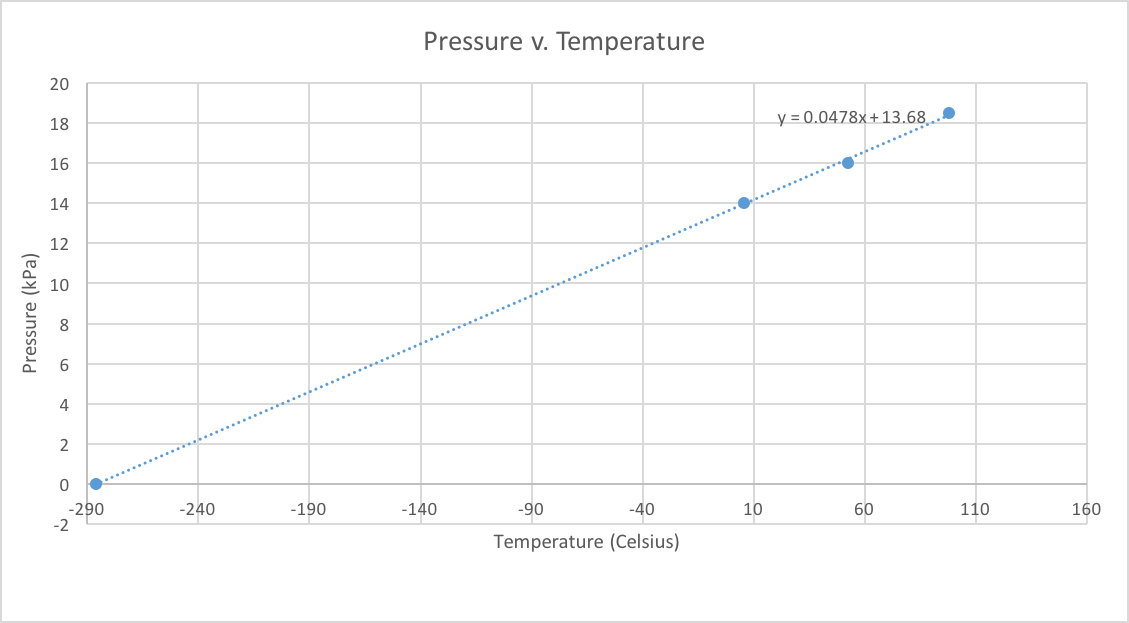
\includegraphics[scale=.4]{P_vs_T.png}
    \caption{Linear regression model of temperature versus pressure with constant volume}
    \label{P_vs_T}
  \end{figure}

  The linear regression shows that, using the collected data, absolute zero temperature in Celsius is -286.22$^{\circ}$C. There is an error margin of 4.8$\%$ when compared to the known value of absolute zero, -273.15$^{\circ}$C.

  \section{Discussion}

	The first part of the experiment utilized the procedure mentioned above in an attempt to demonstrate the linear relationship between volume and temperature. The results of this experiment indicate that absolute zero temperature is -648.8$^{\circ}$C, determined by finding the x-intercept of the linear regression model. There is an error margin of 237.5$\%$ when compared to the known value of absolute zero, -273.15$^{\circ}$C. This experimental value initially suggests the relationship between volume and temperature is not linear and that the ideal gas law is invalid. However, experimental errors were likely to have occurred, resulting in this significantly large margin of error. These include, but are not limited to, not waiting long enough for the temperature to equalize before taking measurements, poor plumbing when measuring the volume when running steam through the pipe, resulting in an insufficient amount of steam while taking the final measurement, and --- the most probable cause --- bad entry of the data during analysis. Table 1 clearly shows identical values for steam and warm water to three significant figures, implying that the same experimental value was accidentally entered into the analysis for both conditions.

	Part two of the experiment utilized the procedure mentioned above to demonstrate the linear relationship between pressure and temperature. The results of this experiment show that absolute zero temperature is -286.88$^{\circ}$C. There is an error margin of 4.8$\%$ when compared to the known value of absolute zero -273.15$^{\circ}$C. This experimental value suggests the relationship between pressure and temperature is indeed linear and that the ideal gas law is valid. Experimental error may have come from not waiting long enough for the metallic sphere temperature to equalize with the water when it was boiling. The pressure reading was taken with a temperature reading 97.8$^{\circ}$C. While the water was visibly boiling, this deviation may have been large enough to introduce error.

  \section{Conclusion}

  Part one of this experiment failed to confirm the linearity of the ideal gas law. This deviation from the model appears to be due to a bad high-temperature measurement, and resulted in a gross underestimation of zero Kelvin. In addition, it imposed an apparently nonlinear shape on the data. Qualitatively examining the first three data points in isolation shows the potential for a high degree of linearity. To avoid this kind of error in future experiments, the authors recommend allowing more time for the steam to condensate around the inner chamber, and a closer attention to detail during data entry.

  In contrast, part two of the experiment agreed quite closely with both the model and the linear fit. The absolute zero approximation differed only slightly (4.8$\%$) from the well-established value, and the data showed a high degree of linearity. As mentioned in the discussion, future experiments should seek to reach true boiling point before recording in order to minimize error.


  \section{Appendix}

  \begin{enumerate}
    \item This value was calculated using the following expression:
    $$t_{\text{absolute zero} } = \dfrac{(t_b - t_f)(-P_f)}{P_b-P_f}$$
    where subscripts f and b represent freezing and boiling, respectively.
  \end{enumerate}

  \begin{table*}[h]
    \centering
    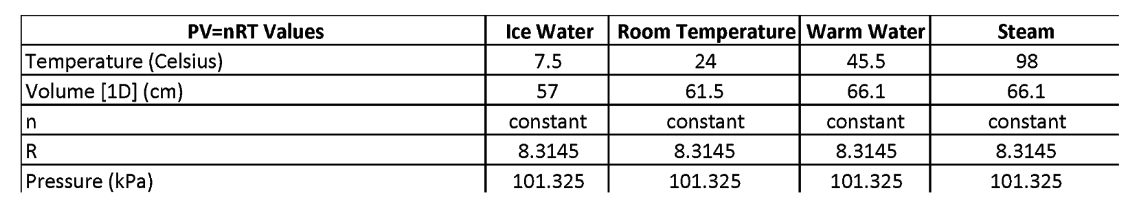
\includegraphics[scale=.4]{table1.png}
    \caption{Data recorded during experiment 1.}
    \label{t1}
  \end{table*}

  \begin{table*}[h]
    \centering
    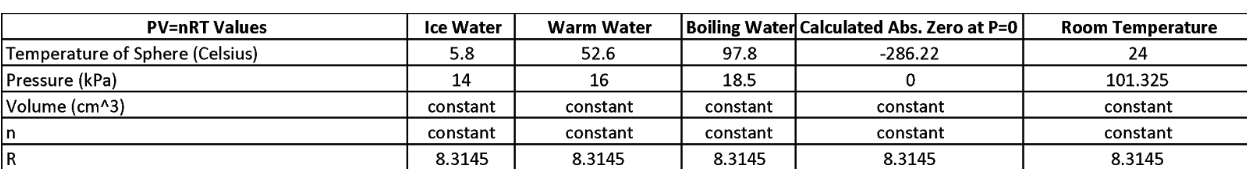
\includegraphics[scale=.4]{table2.png}
    \caption{Data recorded during experiment 2, in addition to the resultant approximation for zero Kelvin with respect to Celsius.}
    \label{t2}
  \end{table*}

\end{document}
